\section{Introduction}

This \cgal\ component implements two surface reconstruction methods which take as input unorganized point sets and compute an implicit function. The output surface mesh is generated by extracting an isosurface of this function with the \cgal\ Surface Mesh Generator~\cite{cgal:ry-gsddrm-06} or any other surface contouring algorithm. \\

More specifically, the input is an unorganized point set, possibly with attributes such as unoriented normals or oriented normals. This point set can be analyzed to measure common statistics quantities and bounding volumes such as average spacing, centroid, bounding box and bounding sphere. We can furthermore pre-processed the point set before reconstruction with dedicated functions devoted to reduction, smoothing, outlier removal, normal estimation and normal orientation.\\

The core surface reconstruction algorithms consist of computing implicit functions which are either an approximate signed distance function to the inferred surface (Algebraic Point Set Surface - referred to as APSS in the sequel) or an approximate indicator function of the inferred solid (Poisson Surface Reconstruction - referred to as Poisson). Another distinction between the APSS and Poisson algorithms lies into the fact that APSS evaluates the function on the fly at any point location while Poisson requires solving for the implicit function before evaluation. The component is structured along a surface reconstruction pipeline that we now detail. 

% Insert image introduction.jpg/eps
\begin{center}
    \label{Surface_reconstruction_3-fig-introduction}
    % Image
    \begin{ccTexOnly}
        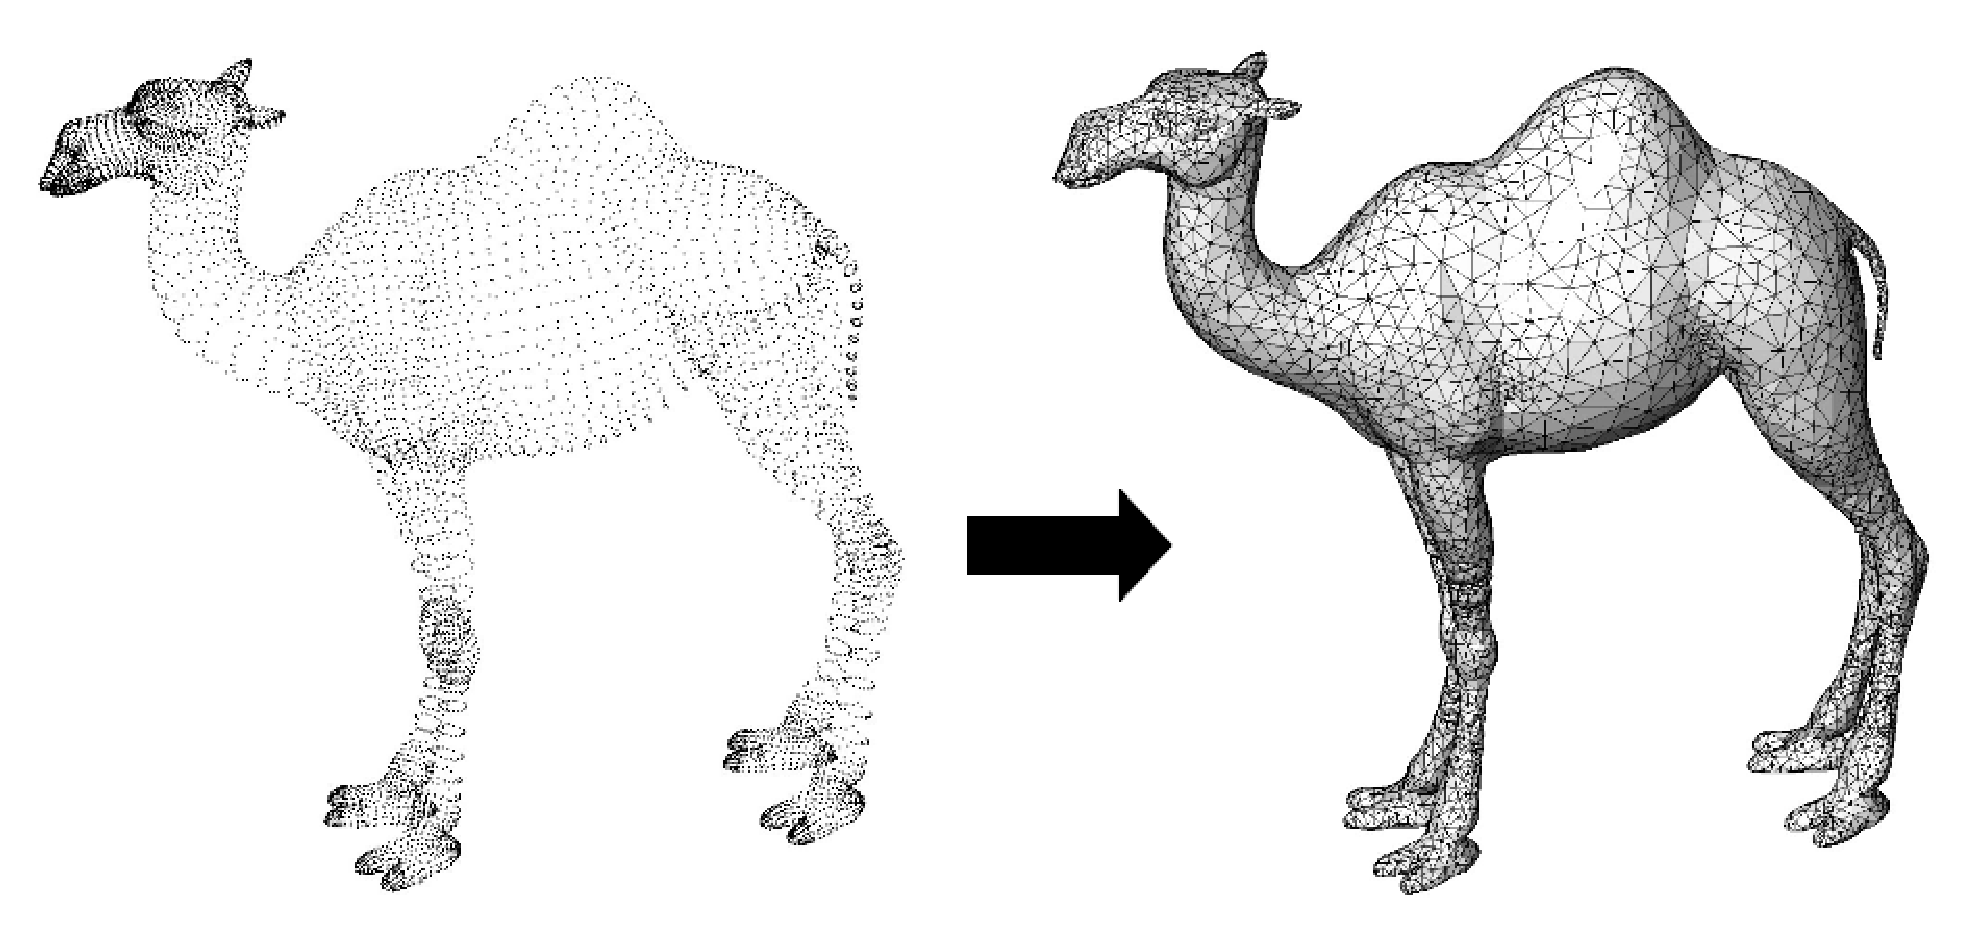
\includegraphics[width=0.9\textwidth]{Surface_reconstruction_3/introduction} % omit .eps suffix
    \end{ccTexOnly}
    \begin{ccHtmlOnly}
        <img width="90%" border=0 src="./introduction.jpg"><P>
    \end{ccHtmlOnly}
    % Title
    \begin{figure}[h]
        \caption{Surface reconstruction from point set}
    \end{figure}
\end{center}

\subsection{Pipeline}

\subsubsection{Input}

\begin{itemize}
\item 3D points
\item 3D points with unoriented normals
\item 3D points with oriented normals
\end{itemize}


\subsubsection{Analysis}

\begin{itemize}
\item Point set barycenter, bounding box, bounding sphere (provided by \cgal\ Principal Components Analysis package)
\item Average spacing to the K nearest neighbors
\end{itemize}


\subsubsection{Processing}

Outlier removal:

\begin{itemize}
\item Outlier removal wrt average squared distance to the K nearest neighbors
\end{itemize}

Point set simplification:

\begin{itemize}
\item Point set simplification by clustering
\item Random point set simplification
\end{itemize}

Smoothing:

\begin{itemize}
\item Smoothing via Jet fitting over the K nearest neighbors + reprojection
\end{itemize}

Normal estimation:

\begin{itemize}
\item Normal estimation by Principal Components Analysis over the K nearest neighbors
\item Normal estimation by Jet fitting over the K nearest neighbors
\end{itemize}

Normal orientation:

\begin{itemize}
\item Normal orientation using a Minimal Spanning Tree \cite{cgal:hddms-srup-92}
\end{itemize}


\subsubsection{Surface Reconstruction}

Implicit functions:

\begin{itemize}
\item Delaunay-based Poisson reconstruction \cite{Kazhdan06}
\item Algebraic Point Set Surfaces \cite{Guennebaud07}
\end{itemize}

Implicit function contouring:

\begin{itemize}
\item \cgal\ Surface Mesh Generator~\cite{cgal:ry-gsddrm-06,cgal:bo-pgsms-05}
\end{itemize}


\subsubsection{Output}

\begin{itemize}
\item 2-manifold surfaces vs non-manifold surfaces
\item Watertight models vs models with boundaries
\item The general case is just: a polygon soup
\end{itemize}


